\documentclass{article}
\usepackage{graphicx}
\usepackage{float}
\usepackage{booktabs}
\usepackage{siunitx}
\usepackage[fleqn]{amsmath}

\title{Lab 2: Getting started with Ohm's Law, KVL, KCL, and Multi-Meter
Measurements}
\author{Sean Balbale}
\date{September 9th, 2023}
\setlength{\parindent}{0in}

\begin{document}

\begin{titlepage}
	\begin{center}
		\vspace*{1in}

		\Huge
		\textbf{Lab 3}

		\LARGE
		Basic Instruments, Components and Circuits. Introduction to KVL, KCL, and LTSpice

		\vspace{3 in}

		\textbf{Student Name:} Sean Balbale
		\\ \textbf{Instructor:} Dr. Iman Salama
		\\ \textbf{Lab Partner Name:} Krish Gupta
		\\ \textbf{Date:} September 25, 2024

		\vfill


	\end{center}
\end{titlepage}

\newpage


\section{Introduction}
The purpose of this lab was to introduce students to key circuit analysis principles 
and tools, specifically Kirchhoff's Voltage Law (KVL), Kirchhoff's Current Law (KCL), 
and LTSpice simulation software. These were fundamental in understanding and designing 
electrical circuits, which are essential for various applications, including biomedical 
engineering. 
\newline

In this lab, students worked with basic components such as resistors, voltage sources, 
and current sources. They also familiarized themselves with LTSpice, a widely used 
circuit simulation tool that allowed for both schematic design and circuit analysis. 
This lab provided hands-on experience in setting up and analyzing DC circuits, as 
well as verifying KCL and KVL through simulation results. Additionally, the lab 
encouraged troubleshooting and iterative design, which are critical skills for engineers. 
The experience gained was essential for future labs and coursework throughout the semester.
\newline

The experiment also aimed to ensure a practical understanding of the function and use 
of basic instruments and circuit components in electrical engineering. By simulating 
various circuit configurations and observing real-time data, students gained insights
 into the accuracy and effectiveness of theoretical laws in real-world applications.

\section{Results}


\subsection{LTSpice Modeling}

\begin{figure}[H]
	\centering
	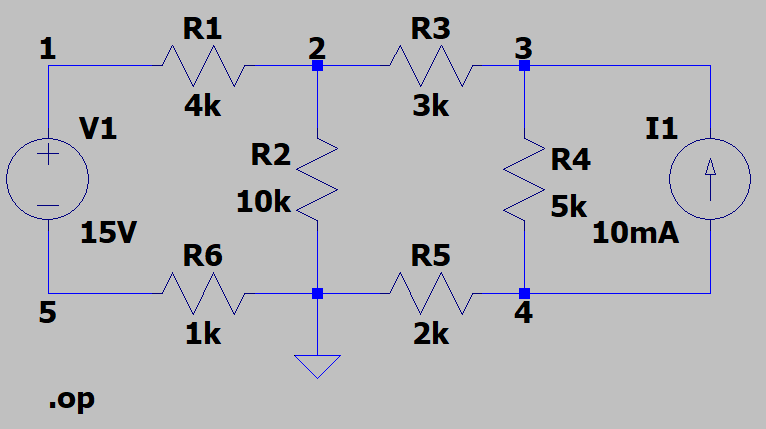
\includegraphics[width=0.5\textwidth]{Lab 3 Circuit.PNG}
	\caption{Lab 3 Circuit}
	\label{fig:fig1}
\end{figure}

During this lab section, the circuit shown in (Figure~\ref{fig:fig1}) was designed and simulated using LTSpice.

\subsection{Verifying Kirchoff's Laws}
\subsubsection{Kirchoff's Current Law (KCL)}
The KCL was verified by analyzing the current at each node in the circuit. 
The sum of currents entering a node was equal to the sum of currents leaving the 
node. This was confirmed by the simulation results in LTSpice.

\begin{equation}
    \begin{split}
        2: R_{1} + R_{2} + R_{3} = 1 + 2  + -3 = 0 \\
        3: R_{4} + R_{3} + I_{1} = 3 + 7  + -10 = 0 \\
        4: R_{4} + R_{5} + I_{1} = 7 + 3  + -10 = 0 \\
        \text{Ground}: R_{2} + R_{6} + R_{5} = -2 + -1 + 3 = 0
    \end{split}
\end{equation}

As seen in the calculations above, the sum of currents at each node was equal to zero, thus verifying KCL.
\newline

If the voltage source was changed to -15V, and the current source was changed to -10mA, KCL would still be valid.
The values of the currents would change, but the sum of currents at each node would still be zero.

\subsubsection{Kirchoff's Voltage Law (KVL)}
The KVL was verified by analyzing the voltage drops across each loop in the circuit.
The voltages around each of the loops were equal to zero.
This was confirmed by the simulation results in LTSpice.
\newline

The following loops were tested:
$V_1 - R_1 - R_2 - R_6$, $R_2 - R_3 - R_4 - R_5$, and $V_1 - R_1 - R_3 - I_1 - R_5 - R_6$.
\newline

The voltage drops across each loop were calculated as follows:
\begin{equation}
    \begin{split}
        &\text{Loop 1: } V_1 - R_1 - R_2 - R_6 = (16-20) + (20-0) + (0-1) + (1-16) = 0 \\
        &\text{Loop 2: } R_2 - R_3 - R_4 - R_5 = (0-20) + (20-29) + (29--6) + (-6-0) = 0 \\
        &\text{Loop 3: } V_1 - R_1 - R_3 - I_1 - R_5 - R_6 = (1-16) + (16-20) \\
            & \; + (20-29) + (29--6) + (-6-0) + (0-1) = 0
    \end{split}
\end{equation}

As seen in the calculations above, the sum of voltage drops around each loop was equal to zero, thus verifying KVL.

\subsection{AC Circuits}
A Keysight Function Generator was used to generate a 10Hz square wave with a 5V peak-to-peak amplitude. The output was
connected to a Keysight Oscilloscope to confirm the waveform. The oscilloscope was set to high Z mode to produce the set waveform.

\begin{figure}[H]
	\centering
	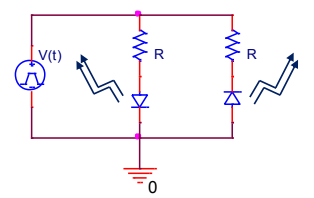
\includegraphics[width=0.5\textwidth]{Blinking LED Circuit.png}
	\caption{Blinking LED Circuit}
	\label{fig:fig2}
\end{figure}

The circuit shown in (Figure~\ref{fig:fig2}) was designed to blink an LED using the square wave generated by the function generator. 
The LED was connected to the output of the function generator through a resistor. Since the LEDs are connected in parallel, the two 
leds will blink at the same time. The LED will blink at the frequency of the square wave. As the frequency decreases, the blinking 
slows down and vice versa.
\newline

If the waveform of the square wave was changed to a sine wave, the LED would still blink. However, the blinking pattern would be
smoother. The LED would turn on and off gradually as the sine wave changes. The blinking would be less abrupt compared to the square wave.
The same goes for if the waveform was changed to a triangle wave. The LED would still blink, but the blinking pattern would be different.
The LED would turn on and off gradually as the triangle wave changes. The blinking would be less abrupt compared to the square wave.
\newline

The highest frequency where the LED was still blinking was 42Hz regardless of the waveform. After that frequency, the LED would looks like it is on all the time.
This frequency is different for different people because of the fact that the human eye can only see up to a certain frequency and their brain can only
process information so quickly. If someone can see up to 60Hz, then the LED would look like it is on all the time after 60Hz. If someone can see up to 30Hz, 
then the LED would look like it is on all the time after 30Hz. 
\newline

If the amplitude of the square wave was changed to 10V, the LED would still blink. The brightness of the LED would increase because the voltage across the LED
would increase. The LED would turn on and off at the same frequency as before, but the brightness would be different. The LED would be brighter at 10V compared to 5V.
This will effect the max frequency that the LED can blink at. The LED would look like it is on all the time at a at a lower frequency compared to 5V because 
the LED would be brighter at 10V compared to 5V.


\section{Discussions and Conclusions}
The lab saw a successful verification of Kirchhoff’s Current Law (KCL) and Kirchhoff’s Voltage Law (KVL), 
realized through both theoretical computations and LTSpice simulations. The conclusions from the simulations 
were in agreement with the expectations from the laws, strengthening the validity of LTSpice as a tool for the
 analysis of circuits.
\newline

The verification of KCL was simple since the total currents entering versus those leaving every node were found 
to be zero. This showed that LTSpice deals with current directionality effectively and furnishes simulated data 
that is reliable for node analysis. In a like manner, KVL was confirmed by investigating the combined voltage drops 
along various closed circuits, all of which added up to zero as dictated by the law. The exercise showed practical 
evidence for theoretical circuit laws, proving that LTSpice can prevail as a valuable tool for modelling real electrical systems.
\newline    

Through the function generator and oscilloscope configuration, students were able to see the behavior of various 
waveforms in an LED circuit for AC circuits. Depending on the waveform frequency, the LED blinking frequency was 
highly variable. As predicted, the square wave created abrupt on/off transitions, in contrast, the sine and triangle 
waves yielded smoother transitions, which emphasized the variations in how these waveforms function in a circuit. 
This confirmed the critical nature of waveform selection in the design of circuits, particularly in applications that
 involve precise timing such as blinking indicators and signal modulation.
\newline

The study further demonstrated that the perceived blinking frequency was inconsistent between individuals, 
which we can attribute to the constraints of human vision perception. This finding brings to light an 
important consideration in the design of visual signal indicators or user interface components that contain 
frequency-based visual stimuli. In addition, the findings on the relationship between waveform amplitude and 
LED brightness showed the immediate association between voltage and light intensity in LEDs, key for settings 
that need adjustable brightness settings.
\newline

Participants in this lab obtained important practical knowledge in the use and validation of Kirchhoff's laws 
through both theoretical calculations and LTSpice simulations. The results confirmed that these laws provide an 
accurate prediction of electrical circuit behavior. In addition, utilizing LTSpice as a simulation tool was effective 
for the purpose of modeling elaborate circuits, an important skill in electrical engineering.
\newline

The research into AC circuits with differing waveforms confirmed that waveform shape and frequency alter circuit 
behavior, primarily regarding timing and the management of brightness. Observations from this experiment will be 
vital for labs to come, where they will study more complicated circuits and simulations. The lab, in general, was 
fruitful in increasing both understanding of theory and practical capabilities in circuit analysis.


\section{References}
 [1] Dr. Iman Salama. “Lab 3 – Basic Instruments, Components and Circuits.
 Introduction to KVL, KCL, and LTSpice” Northeastern University. 25 September 2024.

\end{document}
